\title{STA 602 HW2}
\documentclass[11pt, letterpaper]{article}
\usepackage[utf8]{inputenc}
\usepackage[letterpaper, margin=0.5in]{geometry}
\usepackage{amsmath}
\usepackage{amssymb}
\usepackage{amsthm}
\usepackage{graphicx}
\usepackage[font=scriptsize]{caption}
\usepackage{subcaption}
\graphicspath{ {.} }
\captionsetup{justification=raggedright, singlelinecheck=false}

\author{Ryan Tang}
\date{October 7th 2022}

\begin{document}
\maketitle

\section{HW4 Exercise 3}
\paragraph{(d)}
Now instead of plotting MSE, here we estimated MAE using Monte Carlo. Still the exact 5 estimators, below are the MAE comparisons (Figures 5 and 6). I noticed that the loss function is no longer convex; many humps can make optimization stuck in local maxima. It is espcially visible with a small sample size. However, the general Bayesian update behaviors stay directionally similar between L2 and L1. L1 is just a sharper and rigid. Lastly, it looks like the $\delta_5$ L2 minimax estimator is still a minimax estimator in the L1 context.
\begin{figure*}[!h]
  \centering
  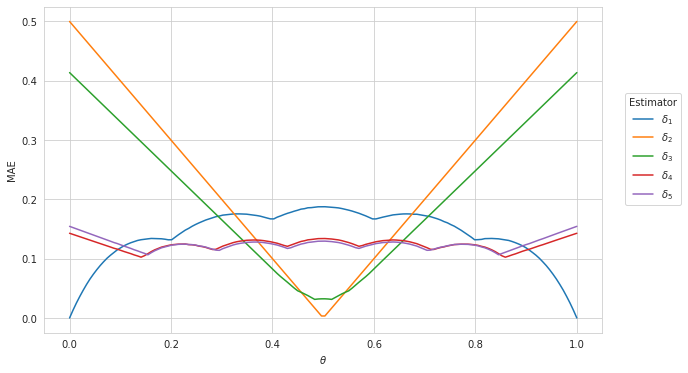
\includegraphics[width=0.7\textwidth]{3.d.1.png}
  \captionsetup{justification=centering}
  \caption{Political Poll MAE Comparison, $n = 5$}
\end{figure*}

\begin{figure*}[!h]
  \centering
  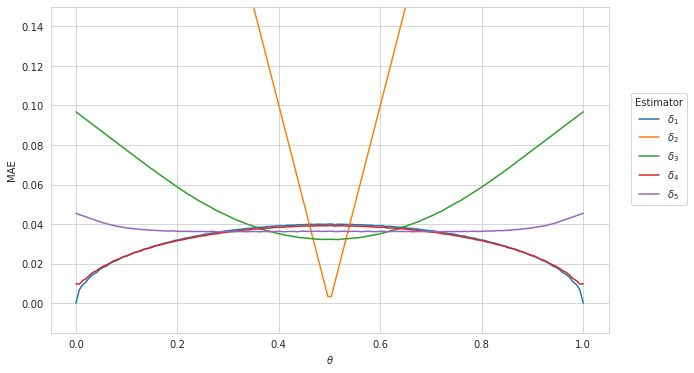
\includegraphics[width=0.7\textwidth]{3.d.2.png}
  \captionsetup{justification=centering}
  \caption{Political Poll MAE Comparison, $n = 100$}
\end{figure*}

\section{Exercise 4.1}
Based on Exercise 3.1, we have the following posterior for $\theta_1$. And assuming a uniform prior for $\theta_2$, a Binomial generating model for $Y_2$, and a sample of 50 with 30 supports for the policy, we can also write $\theta_2$'s posterior in Beta.
\begin{align*}
    \theta_1|Y_1 &\thicksim Beta(57+1, 1+100-57) = Beta(a=58, b=44) \\
    \theta_2|Y_2 &\thicksim Beta(30+1, 1+50-30) = Beta(a=31, b=21)
\end{align*}
Now, after some sampling with MC, we estimated $p(\theta_1 < \theta_2|Y_1, Y_2) = 0.6316$


\section{Exercise 4.2}
\paragraph{(a)}
According to Exercise 3.3, we have the following prior and posterior for groups $A$ and $B$.
\begin{align*}
    \theta_A &\thicksim Beta(120, 10) && \theta_A|\mathbf{y}_A \thicksim Beta(237, 20) \\
    \theta_B &\thicksim Beta(12, 1) && \theta_A|\mathbf{y}_B \thicksim Beta(125, 14)
\end{align*}
Hence, the estimated $p(\theta_B < \theta_A|\mathbf{y}_A, \mathbf{y}_B) = 0.9957$


\paragraph{(b)}
By adjusting the $\theta_B$ prior with the parameter, $n_0$. We can adjust how strong the prior belief is and make it more insensitive to the new survey data the higher it is. Below is a plot of the sensitivity. As we can see, with $n_0$ increases, the posterior $\{\theta_B < \theta_A\}$ stay closer to 50\%. 
\begin{figure*}[!h]
  \centering
  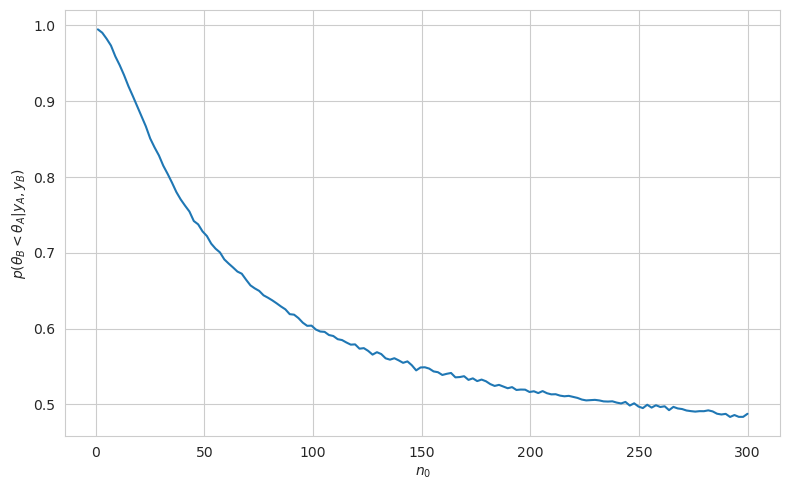
\includegraphics[width=0.7\textwidth]{4.2.b.png}
  \captionsetup{justification=centering}
  \caption{Sensitivity of $\{\theta_B < \theta_A\}$ with respect to $n_0$}
\end{figure*}

\paragraph{(c)}



\section{Exercise 4.4}
\section{Exercise 4.5}
\section{Exercise 4.6}

\end{document}